\documentclass[12pt,letterpaper]{exam}
\usepackage[lmargin=1in,rmargin=1in,tmargin=1in,bmargin=1in]{geometry}
\usepackage{../style/exams}

% -------------------
% Course & Exam Information
% -------------------
\newcommand{\course}{MAT 108: Exam 2}
\newcommand{\term}{Spring --- 2024}
\newcommand{\examdate}{04/01/2023}
\newcommand{\timelimit}{85 Minutes}

\setbool{hideans}{false} % Student: True; Instructor: False

\newcommand{\squiggle}{\rightsquigarrow}

% -------------------
% Content
% -------------------
\begin{document}

\examtitle
\instructions{Write your name on the appropriate line on the exam cover sheet. This exam contains \numpages\ pages (including this cover page) and \numquestions\ questions. Check that you have every page of the exam. Answer the questions in the spaces provided on the question sheets. Be sure to answer every part of each question and show all your work. If you run out of room for an answer, continue on the back of the page --- being sure to indicate the problem number.} 
\scores
\bottomline
\newpage


% -------------------
% Questions
% -------------------
\begin{questions}

% Question 1
\newpage
\question[10] Let $A$, $B$, and $C$ be events from a probability space whose probabilities are given below.
	\[
	\begin{aligned}
	P(A)&= 0.55 \\
	P(B)&= 0.43 \\
	P(C)&= 0.30
	\end{aligned}
	\]

\begin{enumerate}[(a)]
\item Can we say that $P(A \text{ or } B)= 0.55 + 0.43= 0.98$? Explain. 
\item Can we say that $P(A \text{ and } B)= 0.55 \cdot 0.43= 0.2365$? Explain. 
\item Assume that $B$ and $C$ are independent. Find $P(B \text{ or } C)$. 
\item Assume that $B$ and $C$ are disjoint. Find $P(B \text{ and } C)$
\end{enumerate} \pspace

\sol 
\begin{enumerate}[(a)]
\item No, we do not know that $A$ and $B$ are disjoint events. We know $P(A \text{ or } B)= P(A) + P(B)$ for disjoint events but that this may not be the case for events which are not disjoint. We can only say that $P(A \text{ or } B) \leq P(A) + P(B)= 0.55 + 0.43= 0.98$. \pspace

\item No, we do not know that $A$ and $B$ are independent events. We know that $P(A \text{ and } B)= P(A) \cdot P(B)$ if and only if $A$ and $B$ are independent. Therefore, we cannot say that $P(A \text{ and } B)= 0.55 \cdot 0.43= 0.2365$. We would need to if $A$ and $B$ are independent to use $P(A \text{ and } B)= P(A) P(B)$ or know $P(A \;|\; B)$ or $P(B \;|\; A)$ to compute $P(A \text{ and } B)$ using $P(A \text{ and } B)= P(B) P(A \;|\; B)$ or $P(A \text{ and } B)= P(A) P(B \;|\; A)$, respectively. \pspace

\item Because $B$ and $C$ are independent, we know $P(B \text{ and } C)= P(B) P(C)= 0.43 \cdot 0.30= 0.129$. But then\dots
	\[
	P(B \text{ or } C)= P(B) + P(C) - P(B \text{ and } C)= 0.43 + 0.30 - 0.129= 0.601
	\] \pspace

\item Because $B$ and $C$ are disjoint, they cannot occur at the same time. But then\dots
	\[
	P(B \text{ and } C)= 0
	\]
\end{enumerate}



% Question 2
\newpage
\question[15] Statisticians are examining American's satisfaction with the candidates they can vote for in an upcoming election. Each individual surveyed was asked, ``I am satisfied with the options for candidates that I can vote for in the upcoming election.'' An individual could answer `Strongly Disagree', `Disagree', `Neutral', `Agree', or `Strongly Agree.' The gender of each individual was recorded (male, female, or other/refused to disclose). The results are given below. \par
	\begin{table}[ht]
	\centering
	\begin{tabular}{|l|c|c|c|c|c||c|} \hline 
	& Strongly Disagree & Disagree & Neutral & Agree & Strongly Agree & Total \\ \hline \hline
	Male & $15$ & $22$ & $9$ & $4$ & $16$ & $66$ \\ \hline
	Female & $14$ & $26$ & $10$ & $8$ & $11$ & $69$ \\ \hline
	Other/Non-Disclosure & $9$ & $9$ & $4$ & $6$ & $2$ & $30$ \\ \hline \hline
	Total & $38$ & $57$ & $23$ & $18$ & $29$ & $165$ \\ \hline
	\end{tabular}
	\end{table}

\begin{enumerate}[(a)]
\item What percentage of individuals surveyed were not satisfied (strongly disagree or disagree) with the options for candidates in the election? 
\item What percentage of individuals surveyed were female?
\item What percentage of individuals surveyed were neutral or were recorded as either `other gender' or refused to disclose their gender?
\item What percentage of males surveyed strongly agreed with the statement?
\item What percentage of individuals surveyed were females that were neutral about the statement?
\end{enumerate} 

{\footnotesize
\sol 
\begin{enumerate}[(a)]
\item 
	\[
	P(\text{SD or D})= \dfrac{38 + 57}{165}= \dfrac{95}{165} \approx 0.5758
	\]
Therefore, $57.58\%$ of individuals were not satisfied with the options for candidates in the election. 

\item 
	\[
	P(\text{Female})= \dfrac{69}{165} \approx 0.4182
	\] 
Therefore, $41.82\%$ of individuals surveyed were female. 

\item 
	\[
	P(\text{Neutral or Other/ND})= \dfrac{23 + 30 - 4}{165}= \dfrac{49}{165} \approx 0.2970
	\]
Therefore, $29.7\%$ of individuals responded neutrally or were recorded as `other gender' or refused to disclose their gender. 

\item 
	\[
	P(\text{SA} \;|\; \text{Males})= \dfrac{P(\text{SA and Male})}{P(\text{Males})}= \dfrac{16}{66} \approx 0.2424
	\]
Therefore, $55.17\%$ of males strongly agreed with the statement. 

\item 
	\[
	P(\text{Female and Neutral})= \dfrac{10}{165}= 0.0606
	\]
Therefore, $6.05\%$ of individuals surveyed were females that were neutral about the statement. 
\end{enumerate}
}



% Question 3
\newpage
\question[15] A recent study of cholesterol levels for adults in South Korea was determined to be approximately normally distributed with mean 200~mg/dL and standard deviation 50~mg/dL. Based on the results of this survey, answer the following:
        \begin{enumerate}[(a)]
        \item What percentage of adults in South Korea have cholesterol levels less than 136~mg/dL?
        \item What percentage of adults in South Korea have cholesterol levels greater than 232~mg/dL?
        \item What percentage of adults in South Korea have cholesterol levels between 136~mg/dL and 232~mg/dL?
        \item What is the highest cholesterol level an adult in South Korea can have to be in lowest 20\% of cholesterol levels?
        \end{enumerate} 

\sol Based on the results on this survey, the distribution of cholesterol levels in adults in South Korea is $N(\mu, \sigma)= N(200 \text{ mg/dL}, 50 \text{ mg/dL})$. 

\begin{enumerate}[(a)]
\item 
	\[
	z_{136}= \dfrac{136 - 200}{50}= \dfrac{-64}{50}= -1.28 \squiggle 0.1003
	\] 
Therefore, $P(X < 136 \text{ mg/dL})= 0.1003$, i.e. $10.03\%$ of individuals have a cholesterol level of less than 136~mg/dL. \pspace

\item 
	\[
	z_{232}= \dfrac{232 - 200}{50}= \dfrac{32}{50}= 0.64 \squiggle 0.7389
	\] 
But then $P(X > 232 \text{ mg/dL})= 1 - P(X \leq 232 \text{ mg/dL})= 1 - 0.7389= 0.2611$, i.e. $26.11\%$ of individuals have a cholesterol level of greater than 232~mg/dL. \pspace

\item We have\dots
	\[
	\hspace{-2.5cm} P(136 \text{ mg/dL} < X < 232 \text{ mg/dL})= P(X \leq 232 \text{ mg/dL}) - P(X < 136 \text{ mg/dL})= 0.7389 - 0.1003= 0.6386
	\]
That is, $63.86\%$ of individuals have a cholesterol level between 136~mg/dL and 232~mg/dL. \pspace

\item Let $X$ be this highest possible cholesterol level. We know that $X$ is only greater than 20\% of values in the distribution of cholesterol levels. But then $z_X \squiggle 0.20$. Examining the $z$-score chart, we find that $z_X= -0.84$. But then\dots
	\[
	\begin{gathered}
	z_X= -0.84 \\
	\dfrac{X - 200}{50}= -0.84 \\
	X - 200= -42 \\
	X= 158
	\end{gathered}
	\]
Therefore, highest cholesterol level an adult in South Korea can have to be in lowest 20\% of cholesterol levels is 158~mg/dL. 
\end{enumerate}



% Question 4
\newpage
\question[15] Recent TokTik surveys suggest that 15\% of individuals `have the rizz.' An independent, simple random sample of nine individuals was taken. 
        \begin{enumerate}[(a)]
        \item Explain why the count of individuals `having the rizz' in this survey follows a binomial distribution. 
        \item What is the probability that exactly three individuals surveyed `had the rizz'?
        \item What is the probability that at most five but more than two individuals surveyed `had the rizz' ?
        \item What is the probability that at least one individual surveyed `had the rizz.'?
        \end{enumerate} \pspace

\sol 
\begin{enumerate}[(a)]
\item A count needs to meet four criterion to be a given by a binomial distribution:
	\begin{itemize}
	\item The event needs to occur or not with each trial: Each individual surveyed either `has the rizz' or not. 
	\item The probability of observing the even needs to be fixed: We assume there is a fixed 15\% chance that an individual `has the rizz.' 
	\item There needs to be a fixed number of trials: We are examining a fixed survey of size $n= 9$. 
	\item The trials need to be independent: We assume that the individuals surveyed in a way so that whether or not they `have the rizz' is independent from the other individuals.
	\end{itemize}
Therefore, the count, $X$, of individuals in the survey who `have the rizz' is given by a binomial distribution. Specifically, the distribution is $B(n, p)= B(9, 0.15)$. \pspace

\item 
	\[
	P(X= 3)= 0.1069
	\] \pspace

\item 
	\[
	P(2 < X \leq 5)= P(X= 3) + P(X= 4) + P(X= 5)= 0.1069 + 0.0283 + 0.0050= 0.1402
	\] \pspace

\item 
	\[
	P(X \geq 1)= 1 - P(X= 0)= 1 - 0.2316= 0.7684
	\]
\end{enumerate}



% Question 5
\newpage
\question[15] As part of their Clery Act obligations, a university takes a survey of their students to determine their use of illicit substances. The college recorded each student only as male or female and 64\% of individuals surveyed were male. Of the males surveyed, 42\% indicated they had tried an illicit substance on campus, whereas only 23\% of females surveyed answered similarly. 
        \begin{enumerate}[(a)]
        \item What percentage of students surveyed indicated they had used an illicit substance?
        \item What percentage of students surveyed were female or had not tried an illicit substance?
        \item What percentage of students that had tried an illicit substance were male?
        \end{enumerate} \pspace

\sol 
\begin{enumerate}[(a)]
\item 
	\[
	P(\text{Tried})= 0.2688 + 0.0828= 0.3516
	\] 
Therefore, $35.16\%$ of students surveyed indicated they had used an illicit substance. \pspace

\item 
	\[
	P(\text{Female or Not Tried})= 0.3712 + 0.0828 + 0.2772= 0.3712 + 0.36= 0.7312
	\]
Therefore, $73.12\%$ of students surveyed were female or had not tried an illicit substance. \pspace

\item 
	\[
	P(\text{Male} \;|\; \text{Tried})= \dfrac{P(\text{Male and Tried})}{P(\text{Tried})}= \dfrac{0.2688}{0.2688 + 0.0828}= \dfrac{0.2688}{0.3516}= 0.7645
	\]
Therefore, $76.45\%$ of students that had tried an illicit substance were male.
\end{enumerate} \vfill

		\[
		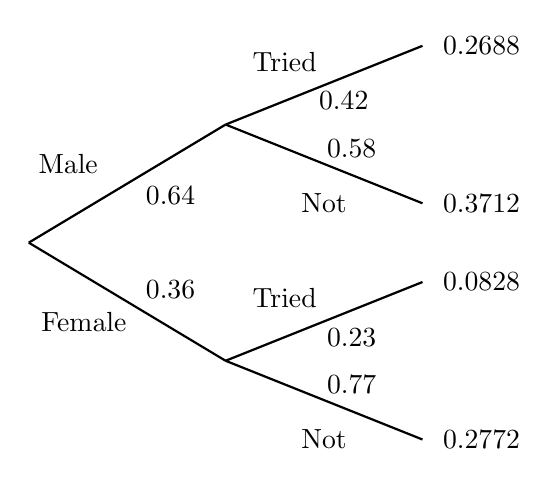
\begin{tikzpicture}[scale= 1.0]
		\def\FirstUpLabel{Male}
		\def\FirstDownLabel{Female}
		\def\SecondUpLabel{Tried}
		\def\SecondDownLabel{Not}
		\def\Up{$0.64$}
		\def\Down{$0.36$}
		\def\UpUp{$0.42$}
		\def\UpDown{$0.58$}
		\def\DownUp{$0.23$}
		\def\DownDown{$0.77$}
		\def\first{$0.2688$}
		\def\second{$0.3712$}
		\def\third{$0.0828$}
		\def\fourth{$0.2772$}
		
		\node at (0.5,1) {\FirstUpLabel};	
		\node at (0.7,-1) {\FirstDownLabel};	
		\node at (1.8,0.6) {\Up};
		\node at (1.8,-0.6) {\Down};
		\draw[thick] (0,0) -- (2.5,1.5);
		\draw[thick] (0,0) -- (2.5,-1.5);
		
		\node at (3.25,2.3) {\SecondUpLabel};
		\node at (3.75,0.5) {\SecondDownLabel};
		\node at (4,1.8) {\UpUp};
		\node at (4.1,1.2) {\UpDown};
		\node at (5.75,2.5) {\first};
		\node at (5.75,0.5) {\second};
		\draw[thick] (2.5,1.5) -- (5,2.5);
		\draw[thick] (2.5,1.5) -- (5,0.5);

		\node at (3.25,-0.7) {\SecondUpLabel};
		\node at (3.75,-2.5) {\SecondDownLabel};
		\node at (4.1,-1.2) {\DownUp};
		\node at (4.1,-1.8) {\DownDown};
		\node at (5.75,-0.5) {\third};	
		\node at (5.75,-2.5) {\fourth};	
		\draw[thick] (2.5,-1.5) -- (5,-0.5);
		\draw[thick] (2.5,-1.5) -- (5,-2.5);
		\end{tikzpicture}
		\]



% Question 6
\newpage
\question[10] A store gets an average of 570~potential customers each day. Past sales records indicate that 17\% of potential customers entering the store each day do not make a purchase. For potential customers that do make a purchase, records indicate that 29\% spend at least \$1 but less than \$100, 33\% spend at least \$100 but less than \$300, and the rest spend at least \$300. What is the smallest average revenue the store should expect to make each day? \pspace

\sol We can first find the average amount spent per customer, i.e. the expected value of a customers expenditure. Because we want the minimal average amount spent per customer, we use the least amount each type of customer will spend on average:
	\[
	\hspace{-1.5cm} EX= \sum x P(x= X)= \$0(0.17) + \$1(0.29) + \$100(0.33) + \$300(0.21)= \$0 + \$0.29 + \$33 + \$63= \$96.29
	\]
Therefore, we expect the smallest average daily revenue to be\dots
	\[
	\begin{aligned}
	\text{Minimal Avg Daily Revenue}&= \text{Number Customers} \cdot \text{Avg. Min. Rev. per Customer} \\
	&= 570 \text{ customers} \cdot \$96.29 \text{/customer} \\
	&= \$54,\!885.30
	\end{aligned}
	\]



% Question 7
\newpage
\question[10] An online retailer sells both PS5 and XBox One. They are examining video game console preferences to determine how many of each console to stock. They survey 120~individuals about which video game console they own. Of the 120 individuals surveyed, 54 stated they owned either a PS5 or an XBox One. Furthermore, 27 stated they only owned a PS5, while 19 stated they only owned an XBox One. 
        \begin{enumerate}[(a)]
        \item What percentage of individuals surveyed owned both a PS5 and an XBox One?
        \item What percentage of individuals surveyed owned neither a PS5 nor an XBox One?
        \item What percentage of individuals surveyed owned an XBox One, if they owned a PS5?
        \end{enumerate} \pspace

\begin{enumerate}[(a)]
\item 
	\[
	P(\text{PS5 and XBox One})= \dfrac{8}{120} \approx 0.0667
	\]
Therefore, $6.67\%$ of individuals surveyed owned both a PS5 and an XBox One. \pspace

\item 
	\[
	P(\text{neither PS5 nor XBox One})= \dfrac{66}{120} \approx 0.55
	\]
Therefore, $55\%$ of individuals surveyed owned neither a PS5 nor an XBox One. \pspace

\item 
	\[
	P(\text{XBox One} \;|\; \text{PS5})= \dfrac{8}{27 + 8}= \dfrac{8}{35} \approx 0.2286
	\]
Therefore, $22.86\%$ of individuals surveyed owned an XBox One, if they owned a PS5, i.e. $22.86\%$ of PS5 owners also owned an XBox One. 
\end{enumerate} \vfill

	\[
	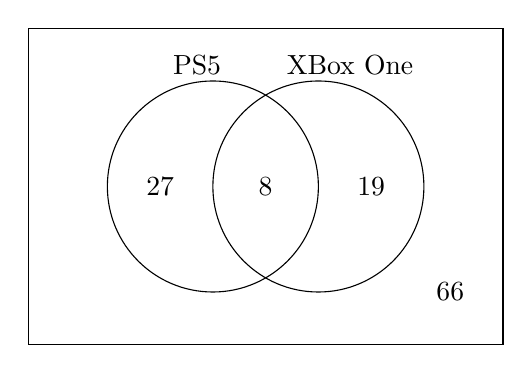
\begin{tikzpicture}[scale=0.67]
	\draw (0,0) rectangle (9,6);
	\draw (3.5,3) circle (2);
	\draw (5.5,3) circle (2);
	
	\node at (3.2,5.3) {PS5};
	\node at (6.1,5.3) {XBox One}; 
	
	\node at (2.5,3) {27};
	\node at (4.5,3) {8};
	\node at (6.5,3) {19};
	\node at (8,1) {66};
	\end{tikzpicture}
	\]



% Question 8
\newpage
\question[10] Economists are studying the effects of inflation on households in the United States. In particular, they examine the change in costs for common household goods. The researchers focus on the city of Chicago. They take a simple random sample of 45~stores in the city and find an average cost of \$2.79 for a gallon of milk. 
\begin{enumerate}[(a)]
\item Explain why the Central Limit Theorem can be used in this situation to examine the distribution of average cost of milk. 
\item Based on the results of this survey, find an 80\% confidence interval for the cost of a gallon of milk in Chicago. [Assume the standard deviation for the cost of a gallon of milk in Chicago is \$0.35.]
\end{enumerate} \pspace

\sol 
\begin{enumerate}[(a)]
\item For the Central Limit Theorem to apply, the sample needs to be a simple random sample, and either the sample has to be `sufficiently large' ($n \geq 30$) or the distribution being sampled from must be normal. We know that the sample was a simple random sample (SRS). While we do not know that the distribution of cost for a gallon of milk in the city of Chicago is normally distributed, we know that the sample size $n= 45 \geq 30$ is `sufficiently large.' Therefore, the Central Limit Theorem applies. \pspace

\item If the confidence interval captures 80\% of the values, this leaves 20\% of the values outside this interval, i.e. 10\% for each end. Therefore, $z^*$ corresponds to $0.80 + 0.10= 0.90$. We find that $z^* \approx 1.28$. But then\dots
	\[
	\begin{gathered}
	\overline{x} \pm z^* \frac{\sigma}{\sqrt{n}} \\[0.3cm]
	\$2.79 \pm 1.28 \cdot \dfrac{\$0.35}{\sqrt{45}} \\[0.3cm]
	\$2.79 \pm 1.28 \cdot (\$0.0521749) \\[0.3cm]
	\$2.79 \pm \$0.07
	\end{gathered}
	\] \pspace
Therefore, based on this sample, there is an 80\% chance that the average cost of a gallon of milk in the city of Chicago is between \$2.72 and \$2.86.\footnote{Strictly speaking, we have an 80\% chance of having constructed a confidence interval that contains the true average cost of a gallon of milk in the city of Chicago.}
\end{enumerate}


\end{questions}
\end{document}